\documentclass[../../../../../main.tex]{subfiles}
\begin{document}

\subsection{Overview of the Graphical User Interface}
The GUI will look something like:
\begin{figure}[H]
	\begin{center}
		\includegraphics[width=0.4\textwidth]{diagrams/UI.mps}
	\end{center}
	\caption{UI Design}
\end{figure}
as showcased in the analysis.

Within \texttt{JavaFX} there is a hierarchy\cite{javafxHierarchy} of a standard GUI components. This is shown below:
\begin{figure}[H]
\begin{center}
\begin{forest}
  for tree={
    align=center,
    parent anchor=south,
    child anchor=north,
    font=\sffamily,
    edge={thick, -{Stealth[]}},
    l sep+=10pt,
    edge path={
      \noexpand\path [draw, \forestoption{edge}] (!u.parent anchor) -- +(0,-10pt) -| (.child anchor)\forestoption{edge label};
    },
    if level=0{
      inner xsep=0pt,
      tikz={\draw [thick] (.south east) -- (.south west);}
    }{}
  }
  [Graphical User Interface
    [Stage
      [Scene
        [Node 1]
        [Node 2]
        [Node 3]
        [...]
      ]
    ]
  ]
\end{forest}
\end{center}
\caption{\texttt{JavaFX} Components Hierarchical Diagram}
\end{figure}
\begin{wrapfigure}{r}{0.4\textwidth} 
	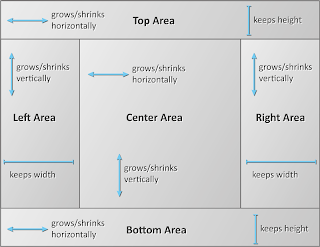
\includegraphics[width=0.4\textwidth]{images/borderpaneArchitecture}
	\caption{\texttt{BorderPane} Architecture}
\end{wrapfigure}
Now we can manipulate the the nodes beneath \texttt{Scene}. It is standard to make the first \texttt{Node} beneath \texttt{Scene} some kind of \texttt{Pane}. For this project a \texttt{BorderPane} is most suited since it has multiple objects of type \texttt{Region}, that can hold one \texttt{Node} each. A diagram of this is shown to the right showcases how a \texttt{BorderPane} is arranged\cite{borderpane} and way it behaves.

The center \texttt{Region} can consist of the plots themselves, and the left \texttt{Region} can consist of the input. The top \texttt{Region} could be used for the ribbon and other buttons to manipulate the plot.
\newpage
\end{document}